\section{Caso 1.a, resistencia interna de la fuente 50 \texorpdfstring{$\Omega$}{Ω}}

Para este caso, las especificaciones indican que la resistencia interna de la fuente de señal es igual a 50 $\Omega$. Por lo tanto, para no cargar la fuente de señal, la impedancia debe ser mucho mayor a este valor, tomamos como criterio que sea 10 veces mas grande.

Luego, los requerimientos de diseño indican que debe tener una ganancia de -30 veces. 
ganancia vo a cada fuente de señal debe ser -30, 

\[ \text { Si: } R_{i}=50 \Omega \Longrightarrow R=10 \space R_{i}=500 \Omega \]
\[ \text { Si }: \quad A_{vm} =-\frac{R_{f}}{R}=-30 \]
\[ \text { Entonces }: \quad R_{f}=15 k \Omega \]
\vspace{1em}



\begin{figure}[h!]
    \centering
    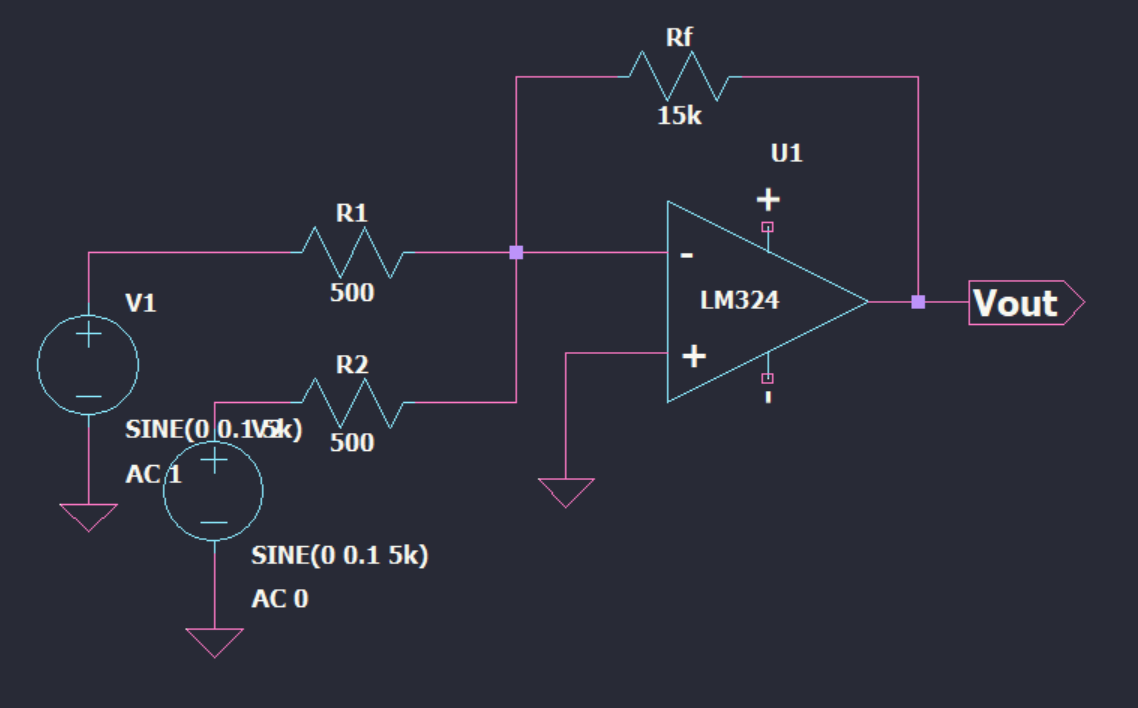
\includegraphics[width=0.90\linewidth]{img/caso1a.png}
    \caption{Esquemático para el caso 1a}
    \label{fig:caso1a}
\end{figure}


\[  \mathbf{R}=500 \Omega, \quad \mathbf{R}_{\mathbf{f}}=15 \mathrm{k} \Omega \]


De esta manera nuestro diseño cumple con las especificaciones de ganancia, impedancia de entrada y valor máximo de resistencias.

\vspace{1em}

\subsection{Errores en DC.}
En primer lugar, obtenemos todos los datos necesarios de la hoja de datos (Figura \ref{fig:caracteristicas}).

\begin{figure}[h!]
    \centering
    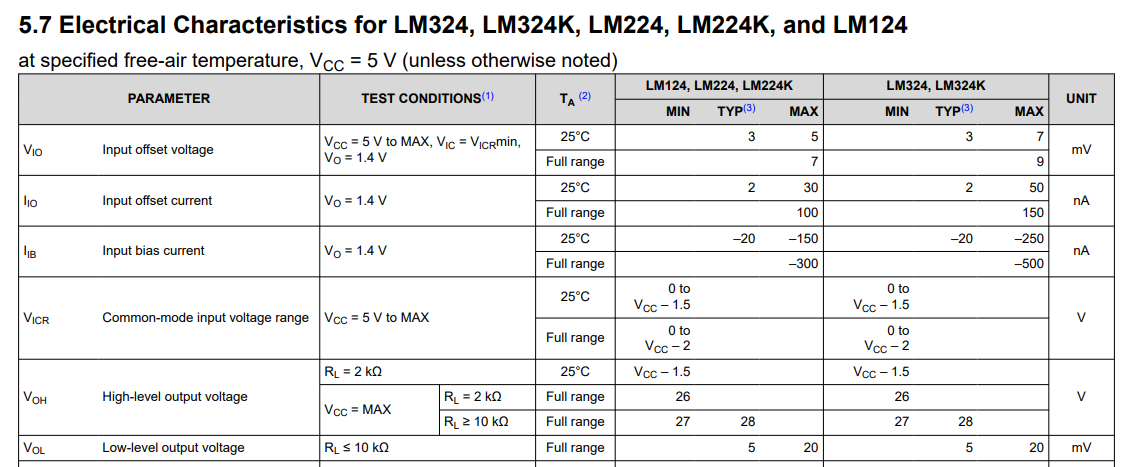
\includegraphics[width=1\linewidth]{img/dc_datasheet.png}
    \caption{Características eléctricas del LM324}
    \label{fig:caracteristicas}
\end{figure}
   
Luego, si reemplazamos por los valores típicos, en las expresiones tenemos que:


\[V_{0} = -30 \cdot (V_1 + V_2) \]
\[T = - Ad   \cdot  \frac{R}{R + 2\cdot R_f} = 100k \cdot \frac{500}{30500} = 1639.3\]

Reemplazando según los datos:
 
\[ \Delta V_{ios} = I_{pol}^{-} \cdot R_f = 20 nF \cdot 15k\Omega = 300 \mu V \]

\vspace{1em}

\[ \Delta V_{os}  = V_{os} \cdot (1 + 2 \cdot \frac {R_f}{R})  =
3mV \cdot 61 = 183 mV \]

\vspace{1em}

\[ \Delta V_{o (Ad)}=\frac{F.S}{\left|T_{o}\right|} = \frac{10V}{1639,39} = 6,1 mV\]

\vspace{1em}

\[ \Delta V_{o (RRMC) } = 0 [ mV ]\]

El error total DC es igual a:

\[ \Delta V_{O} = \Delta V_{ios} + \Delta V_{os} +  \Delta V_{o (A_d)} + \Delta V_{o (RRMC) } = 190 [mV]\]

\subsection{Errores en AC}
 
\subsubsection{Ancho de banda:}

 Primero obtenemos los valores correspondiente a nuestro amplificador de la hoja de datos (figura \ref{fig:1a_slew_rate}).

\begin{figure}[h!]
    \centering
    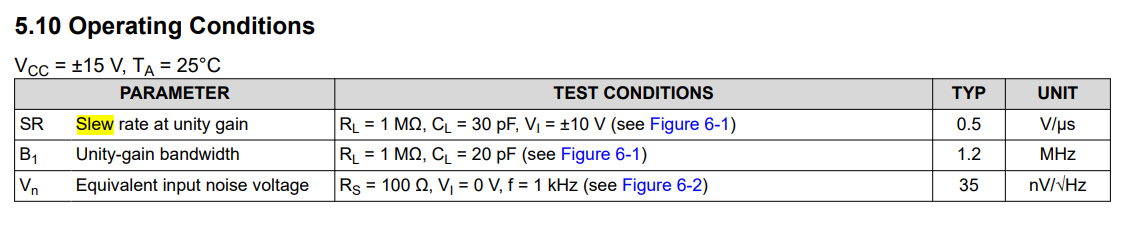
\includegraphics[width=1\linewidth]{img/slewrate_bgw.png}
    \caption{Slew Rate y Producto de ganancia por ancho de banda del LM324}
    \label{fig:1a_slew_rate}
\end{figure}

\[ f_H = f_{T} \frac{R}{R+2 R_f} = 1,2 [MHz] \cdot \frac{500}{30500} = 19,67 [kHz] \]

\subsubsection{Ancho de banda de potencia para 10 \texorpdfstring{$V_{pap}$}{Vpap}:}
\[ f_{Hp}=7,957[\mathrm{kHz}] \]


  
 
\subsection { Ganancia normalizada y error vectorial:}
Se analizaron y tabularon los valores de modulo y fase tanto para la ganancia normalizada como para el error vectorial.

\begin{table}[H]
\centering
\begin{tabular}{|c|c|c|c|c|}
\hline
\rowcolor[HTML]{3fb55b} 
$\omega_h$ & \multicolumn{2}{c|}{avf}         & \multicolumn{2}{c|}{Error Vectorial} \\ \cline{2-5} 
\rowcolor[HTML]{3fb55b}  
           & Mod & Fase (°)     &  Mod & Fase (°)  \\ \hline
 (10\%) & 0.99504 & -5.71059 &  0.00496   & 84.28954 \\ \hline
 (20\%) & 0.98058 & -11.30993 &  0.01942  & 78.69    \\ \hline
 (30\%) & 0.95783 & -16.69924 &  0.04217  & 73.3007  \\ \hline
 (40\%) & 0.92848 & -21.80141 &  0.07152  & 68.19859  \\ \hline
 (50 \%)& 0.89443 & -26.56505 &  0.10557  & 63.43502  \\ \hline
 (60 \%)& 0.85749 & -30.96376 &  0.14251  & 59.03642  \\ \hline
 (70 \%)& 0.81923 & -34.99202 &  0.18077  &  55.00795 \\ \hline
 (80 \%)& 0.78087 & -38.65981 &  0.21913  & 51.34045  \\ \hline
 (90 \%)& 0.74329 & -41.98721 &  0.25671  & 48.01271   \\ \hline
 (100 \%) &  0.70711 & -45.0    &   0.29289  & 45.000    \\ \hline 

\end{tabular}
\caption{Ganancia normalizada y error vectorial}
\label{tabla-error}
\end{table}
En la siguiente grafica podemos observar en color ojo al modulo del error vectorial, y luego en azul podemos observar a la fase del error.
El modulo del error aumenta a medida que aumenta la frecuencia, y la fase disminuye.

\begin{figure}[h!]
    \centering
    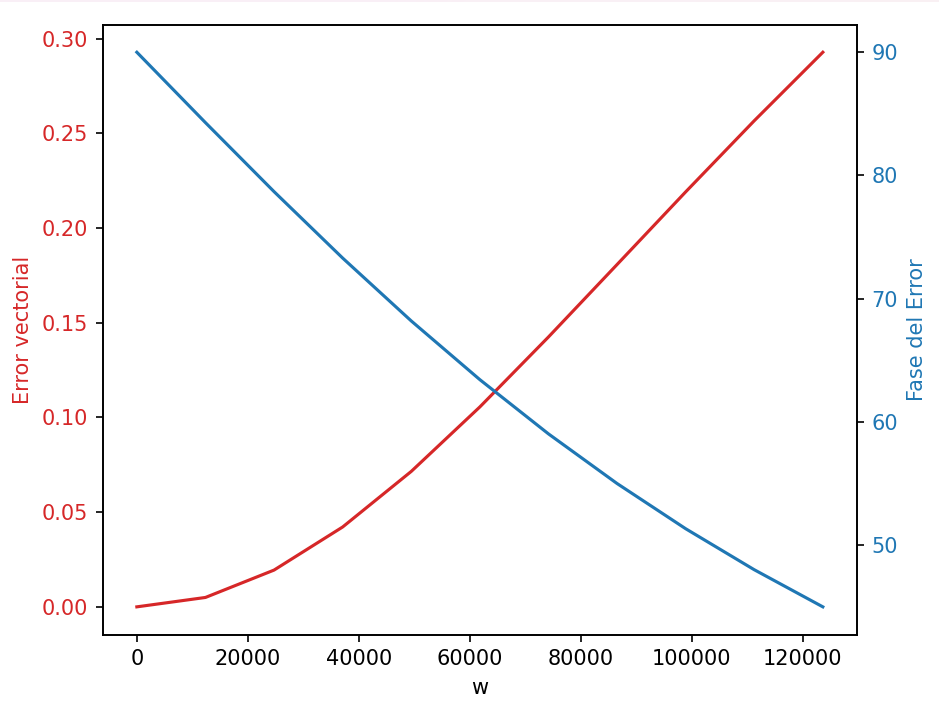
\includegraphics[width=0.80\linewidth]{img/error_vectorial.png}
    \caption{Gráfica error vectorial}
    \label{fig:errorvectorial}
\end{figure}


\newpage
\subsection{Simulaciones}

\subsubsection{Simulación de salida en el tiempo}
 
\begin{figure}[h!]
    \centering
    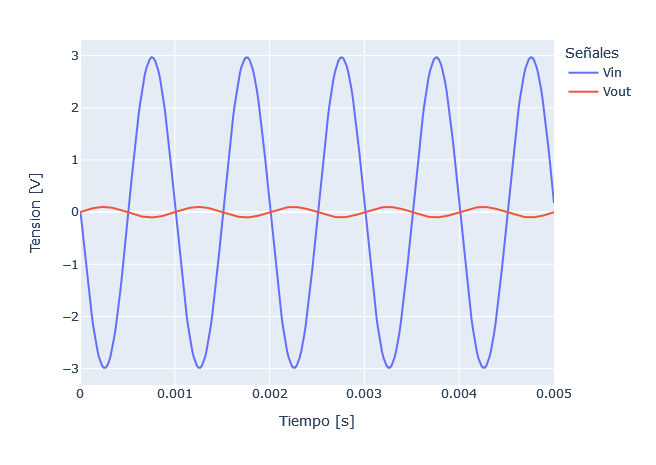
\includegraphics[width=0.80\linewidth]{img/TP2_1_grafico_tiempo.png}
    \caption{Gráfico de voltaje de salida en el tiempo}
    \label{fig:1a_tiempo}
\end{figure}

En esta simulación se puede observar que con una entrada de 100 [mV] a 1 [kHz] obtenemos aproximadamente 3[V] de salida


\subsubsection{Simulación de barrido en frecuencia (bode)}

\begin{figure}[h!]
    \centering
    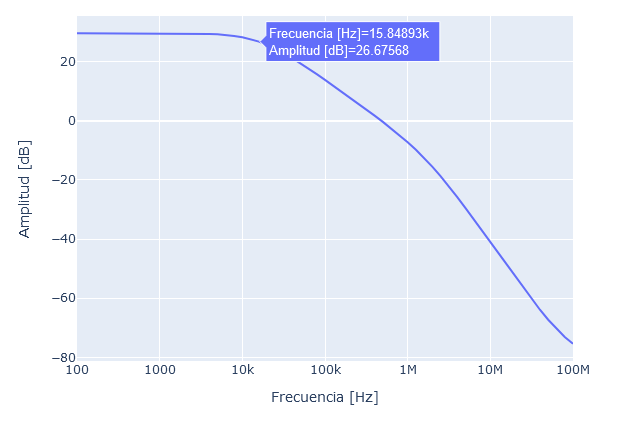
\includegraphics[width=0.80\linewidth]{img/TP2_1_grafico_bode_amp.png}
\end{figure}

\begin{figure}[h!]
    \centering
    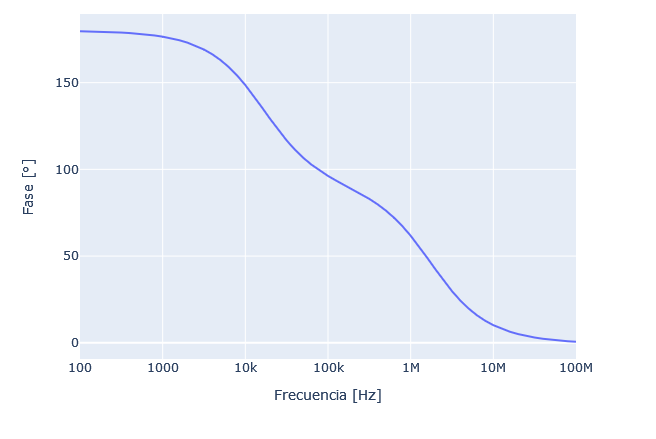
\includegraphics[width=0.85\linewidth]{img/TP2_1_grafico_bode_fase.png}
    \caption{Gráfico de barrido en frecuencia}
    \label{fig:bode1a}
\end{figure}

\subsubsection{Análisis en frecuencia }

Se pueden observar las armónicas de la señal de salida, frente a una señal de entrada de 1kHz.
\begin{figure}[h!]
    \centering
    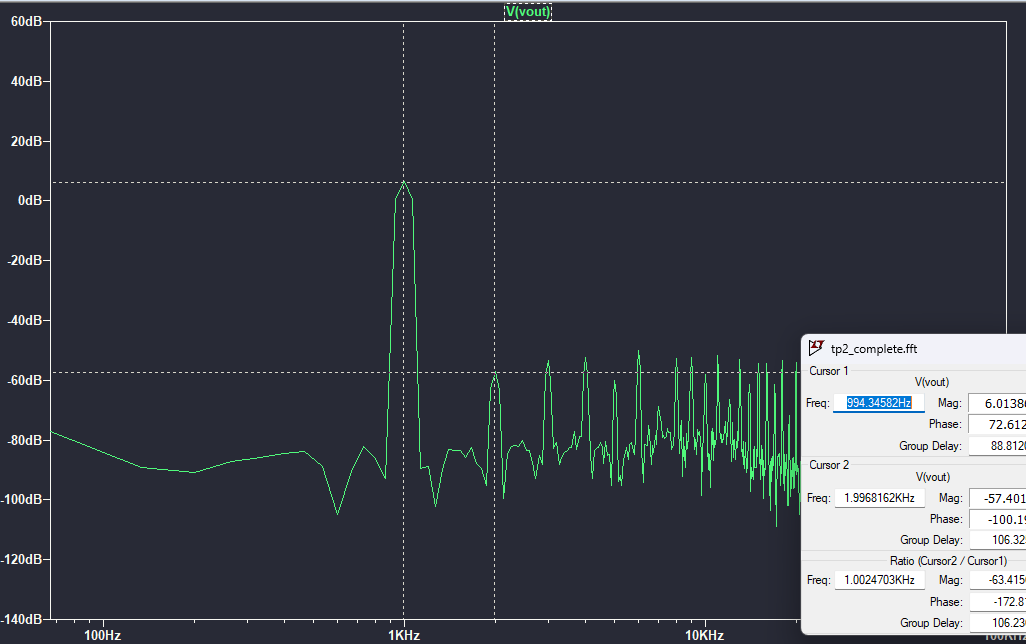
\includegraphics[width=1.0\linewidth]{img/ftt1a.png}
    \caption{Gráfico de la transformada de fourier}
    \label{fig:fft1a}
\end{figure}

\subsection{Mediciones}

\hspace{1mm} Se realizan las mediciones del circuito para el caso de impedancia de entrada 10 veces mayor que la impedancia de la fuente \((Z_{fte}= 50\Omega)\).

\begin{figure}[h!]
    \centering
    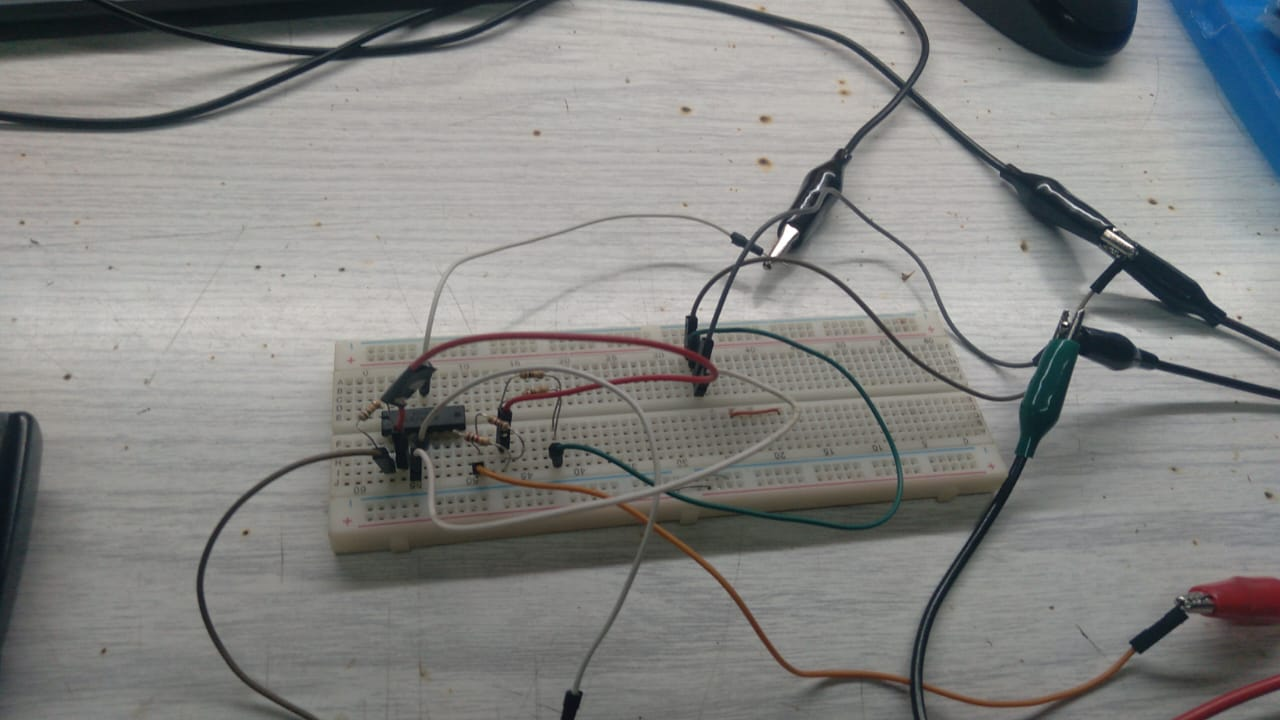
\includegraphics[width=0.80\linewidth]{img/Circuito implementado.jpeg}
    \caption{Circuito implementado}
    
\end{figure}
\begin{figure}[h!]
    \centering
    \includegraphics[width=0.80\linewidth]{img/Una sola señal.jpeg}
    \caption{Inyección de una sola señal}
    
\end{figure}

\begin{figure}[H]
    \centering
    \includegraphics[width=0.3\linewidth]{img/Una sola señal 1.jpeg}
    \caption{Inyección de una sola señal}
    
\end{figure}

\newpage
\hspace{1mm} Se realiza la medición del slew rate.
\begin{figure}[H]
    \centering
    \includegraphics[width=0.8\linewidth]{img/Slew Rate medición.jpeg}
    \caption{Medición de Slew Rate}
    
\end{figure}

Se inyecta una señal escalón al sistema. Luego se mide el tiempo que existe entre el 90\% y el 10\% de la amplitud de la señal de salida. Estos valores no son simétricos.

\[A_{out_{\text{máx}}}= 5V\]
\[A_{out_{\text{mín}}} = -4,5V\] 
\[A_{out_{90\%}}= 4,5V \space y \space A_{out_{10\%}}= -3,6V\]

El tiempo medido es: \(39,6\mu s\). Se calcula entonces el Slew Rate.

\[SR= \frac{9V}{39,6\mu s}= 0,227\frac{V}{\mu s}\]

Comparando con el valor de la hoja de datos, se tiene un valor aproximado ya que el mismo es \(SR= 0,3 \frac{V}{\mu s}\).

Luego se mide el ancho de banda. Se tiene una caída de \(-3~dB\) a la frecuencia \(f_{-3~dB}= 13KHz\).
\begin{figure}[H]
    \centering
    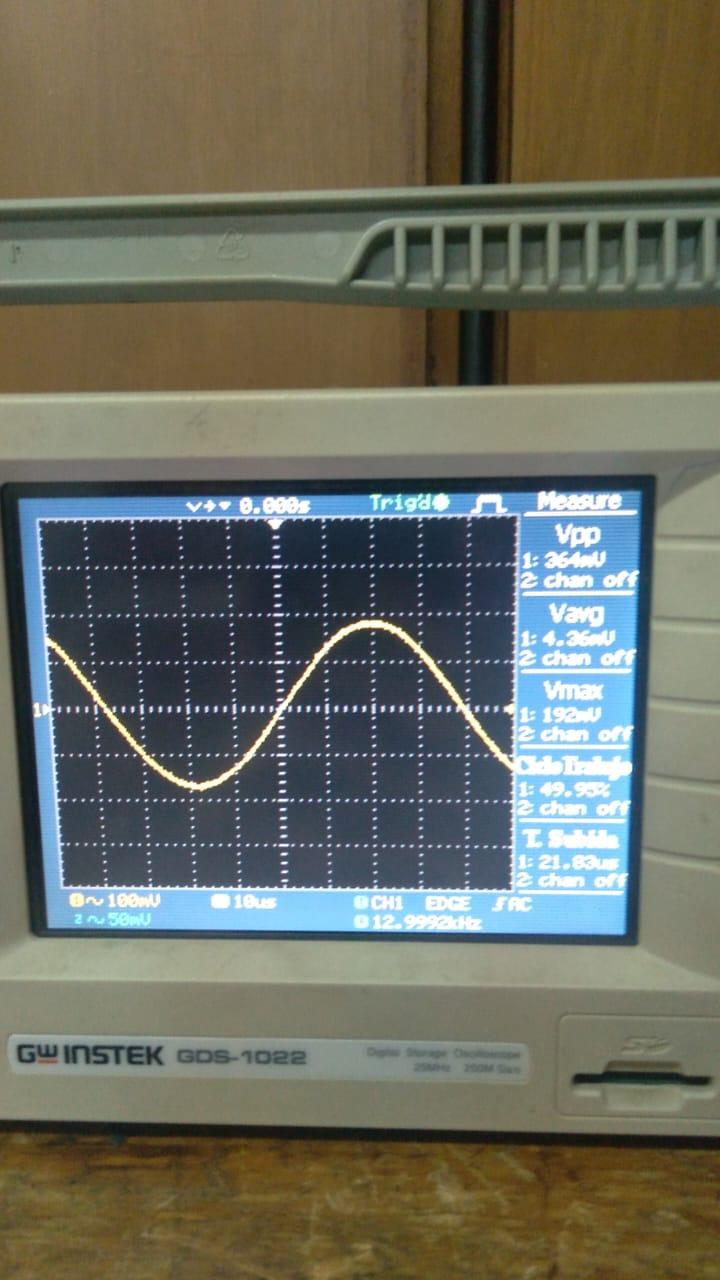
\includegraphics[width=0.8\linewidth]{img/Banda de paso.jpeg}
    \caption{Banda de paso}
    
\end{figure}
\begin{figure}[H]
    \centering
    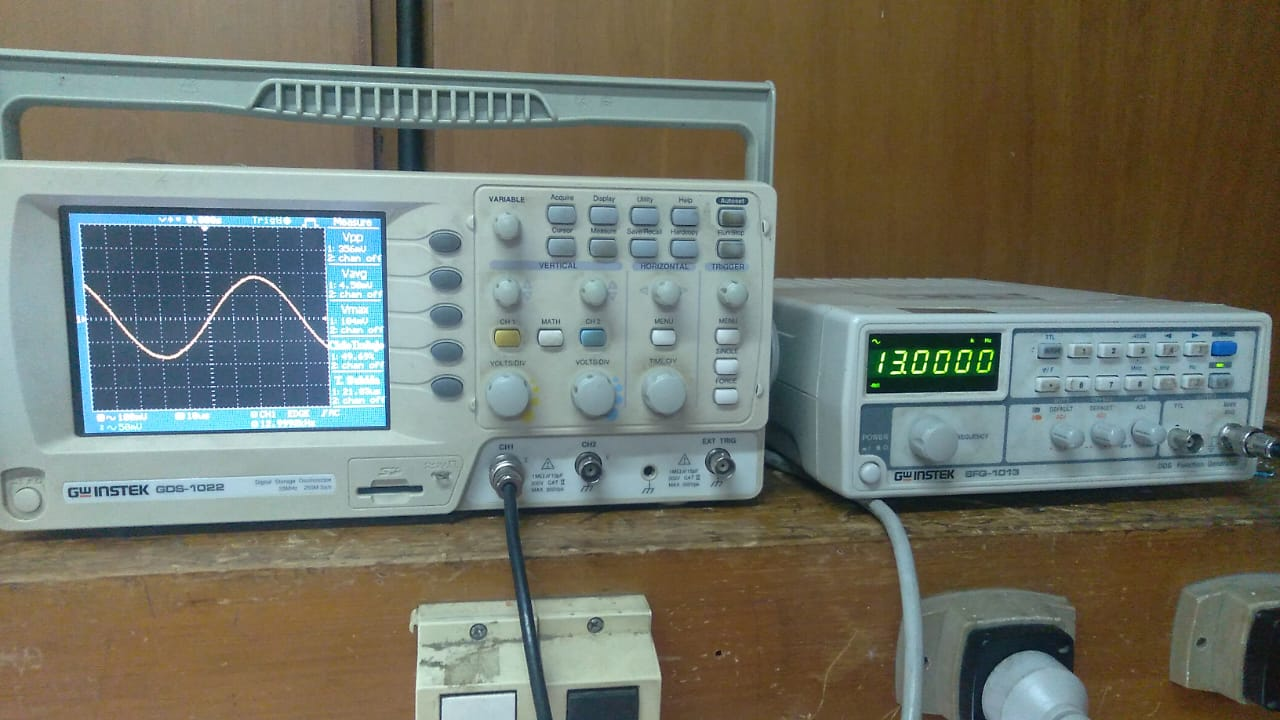
\includegraphics[width=0.8\linewidth]{img/Ancho de banda.jpeg}
    \caption{Frecuencia de caída de -3dB}
    
\end{figure}

Esto mismo se contrasta con la simulación, donde se obtiene una frecuencia \(f_{-3~dB}= 15KHz\) de caída de \(-3dB\).